% This LaTeX was auto-generated from MATLAB code.
% To make changes, update the MATLAB code and export to LaTeX again.

\documentclass{article}

\usepackage[utf8]{inputenc}
\usepackage[T1]{fontenc}
\usepackage{lmodern}
\usepackage{graphicx}
\usepackage{color}
\usepackage{hyperref}
\usepackage{amsmath}
\usepackage{amsfonts}
\usepackage{epstopdf}
\usepackage[table]{xcolor}
\usepackage{matlab}

\sloppy
\epstopdfsetup{outdir=./}
\graphicspath{ {./lgnTUTORIAL_images/} }

\matlabhastoc

\matlabmultipletitles

\begin{document}

\label{T_A48E77F8}
\matlabtitle{Code for assessing local tuning biases in the mouse dLGN}

\begin{itemize}
\setlength{\itemsep}{-1ex}
   \item{\begin{flushleft} perhaps add something that is not the title of your paper, maybe the goal of the paper, or the significance sttament \end{flushleft}}
   \item{\begin{flushleft} link abstract or complete manuscript/thesis \end{flushleft}}
\end{itemize}


\matlabtableofcontents{Table of Contents}

\label{H_BA6C6CEA}
\matlabheading{Goals, Hypothesis and Analysis}

\begin{par}
\begin{flushleft}
The aim of the project is to assess the presence of 'local tuning biases' among populations of LGN afferents innervating the mouse primary visual cortex. 
\end{flushleft}
\end{par}

\label{H_B3487E47}
\begin{par}
\begin{flushleft}
Put simply, we test the notion that groups of LGN neurons  'processing' signals from the same region of visual space do so with a biased set of orientated filters. 
\end{flushleft}
\end{par}

\begin{par}
\begin{flushleft}
To answer this questoin,  
\end{flushleft}
\end{par}

\begin{itemize}
\setlength{\itemsep}{-1ex}
   \item{\begin{flushleft} we Estimate the linear spatial receptive field maps and joint orientation tuning X spatial frequency tuning of populations of thalamic boutons that innervating mouse V1.  \end{flushleft}}
   \item{\begin{flushleft} then For each pair of boutons in the population, find the overlap between the receptive fields the and the similarity of their tuning profiles \end{flushleft}}
   \item{\begin{flushleft} If LGN boutons with overlapping receptive fields have similar tuning profiles, this would suggest the presence of local tuning biases. \end{flushleft}}
\end{itemize}


\label{T_3CE7FFC6}
\matlabtitle{Prepare Data Files}

\begin{matlabcode}
clear;
clc;
cd /Users/luis/Box/prjLGNTB/
addpath /Users/luis/Box/prjLGNTB/lgnDATA/   
addpath /Users/luis/Box/prjLGNTB/lgnANALYSIS/

lgn = lgnanz;
lgn.uif_tbl_base
\end{matlabcode}
\begin{matlabtableoutput}
{
\begin{tabular} {|c|c|c|c|c|}\hline
\mlcell{ } & \mlcell{uif} & \mlcell{mouse\_id} & \mlcell{fname\_base\_ret} & \mlcell{fname\_base\_orisf} \\ \hline
\mlcell{1} & \mlcell{1} & \mlcell{'lgn02'} & \mlcell{'lgn02\_000\_004'} & \mlcell{'lgn02\_000\_003'} \\ \hline
\mlcell{2} & \mlcell{2} & \mlcell{'lgn02'} & \mlcell{'lgn02\_001\_000'} & \mlcell{'lgn02\_001\_001'} \\ \hline
\mlcell{3} & \mlcell{3} & \mlcell{'lgn02'} & \mlcell{'lgn02\_002\_000'} & \mlcell{'lgn02\_002\_002'} \\ \hline
\mlcell{4} & \mlcell{4} & \mlcell{'lgn02'} & \mlcell{'lgn02\_003\_000'} & \mlcell{'lgn02\_003\_001'} \\ \hline
\mlcell{5} & \mlcell{5} & \mlcell{'lgn03'} & \mlcell{'lgn03\_001\_001'} & \mlcell{'lgn03\_001\_000'} \\ \hline
\mlcell{6} & \mlcell{6} & \mlcell{'lgn03'} & \mlcell{'lgn03\_001\_003'} & \mlcell{'lgn03\_001\_002'} \\ \hline
\mlcell{7} & \mlcell{7} & \mlcell{'lgn03'} & \mlcell{'lgn03\_002\_001'} & \mlcell{'lgn03\_002\_000'} \\ \hline
\mlcell{8} & \mlcell{8} & \mlcell{'lgn04'} & \mlcell{'lgn04\_002\_000'} & \mlcell{'lgn04\_002\_003'} \\ \hline
\mlcell{9} & \mlcell{9} & \mlcell{'lgn05'} & \mlcell{'lgn05\_001\_001'} & \mlcell{'lgn05\_001\_000'} \\ \hline
\mlcell{10} & \mlcell{10} & \mlcell{'lgn05'} & \mlcell{'lgn05\_008\_001'} & \mlcell{'lgn05\_008\_000'} \\ \hline
\mlcell{11} & \mlcell{11} & \mlcell{'lgn05'} & \mlcell{'lgn05\_011\_000'} & \mlcell{'lgn05\_011\_001'} \\ 
\hline
\end{tabular}
}
\end{matlabtableoutput}

\begin{par}
\begin{flushleft}
these are all the unique  fields that were imaged. 9 total imaging sessions were conducted, from 4 different mice.
\end{flushleft}
\end{par}


\label{T_CD3E0717}
\matlabtitle{Assessing properties of LGN Boutons}

\label{H_5A5E99C7}
\matlabheading{Load the 'roi' (LGN bouton) data table }

\begin{par}
\begin{flushleft}
discuss implications 
\end{flushleft}
\end{par}

\begin{matlabcode}
uifs_to_process = [3 4];
lgn.get_roi_tables(uifs_to_process);
\end{matlabcode}
\begin{center}
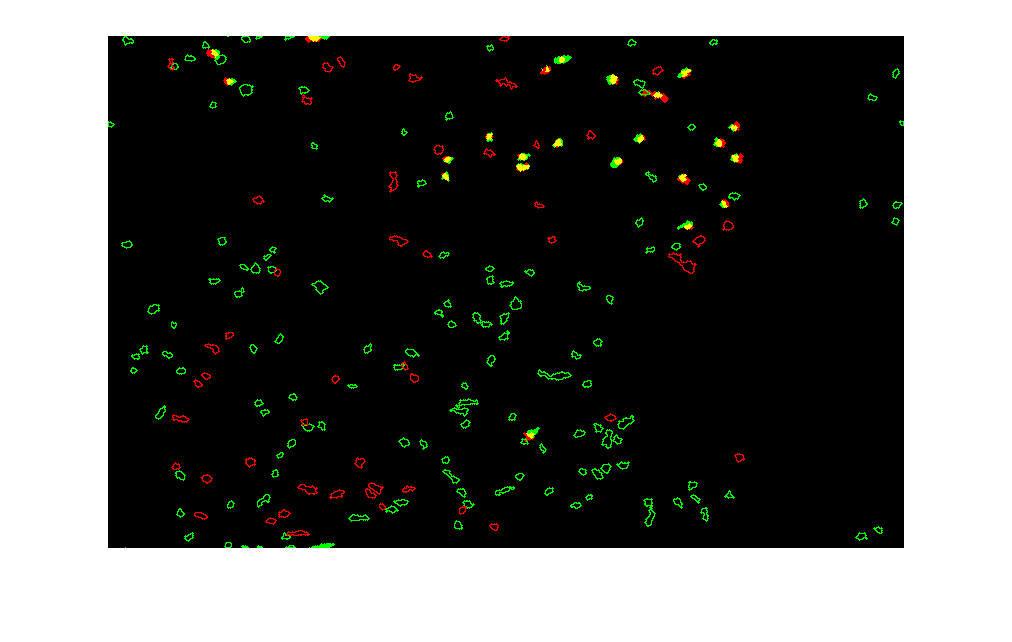
\includegraphics[width=\maxwidth{50.77772202709483em}]{figure_0.png}
\end{center}
\begin{center}
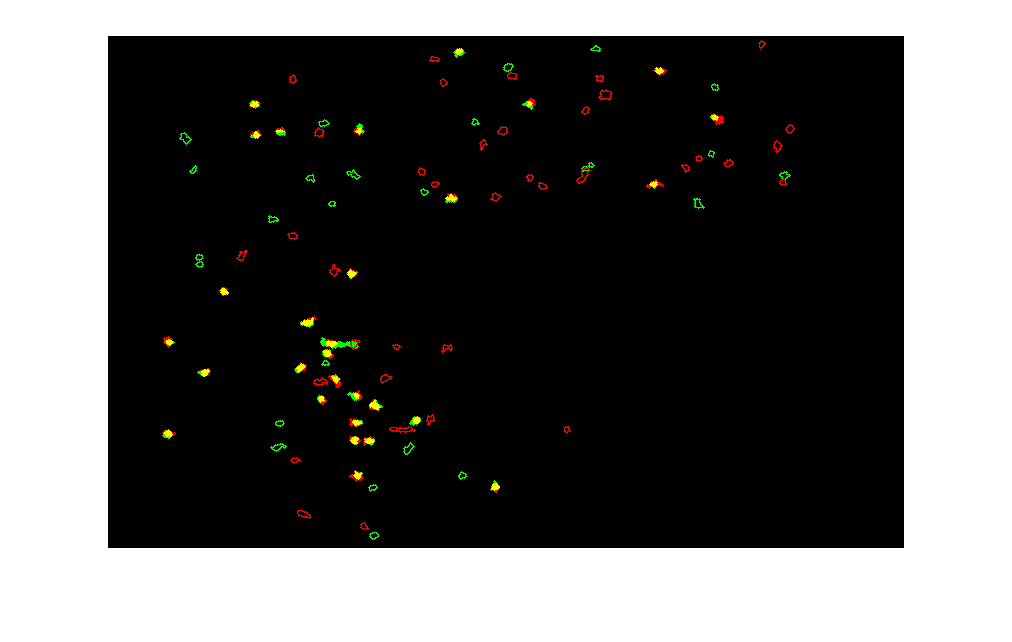
\includegraphics[width=\maxwidth{50.77772202709483em}]{figure_1.png}
\end{center}
\begin{matlabcode}

lgn.roi_stack_uif_list; % here are all all the imaging fields in the roi table
head(lgn.roi_stack) 
\end{matlabcode}
\begin{matlabtableoutput}
{
\begin{tabular} {|c|c|c|c|c|c|c|c|c|c|c|c|c|c|c|c|c|c|c|c|c|c|c|c|c|c|c|c|c|c|c|c|c|c|c|c|c|c|c|c|c|c|c|c|c|c|c|c|c|c|c|c|c|}\hline
\mlcell{ } & \mlcell{masterEntry} & \mlcell{entryNumber} & \mlcell{mouse} & \mlcell{uniqImFieldNum} & \mlcell{hasRetData} & \mlcell{hasTunData} & \mlcell{roi\_ID\_Ret} & \mlcell{roi\_ID\_Tun} & \mlcell{kern\_ret} & \mlcell{kurt\_ret} & \mlcell{sig\_ret} & \multicolumn{2}{|c|}{\mlcell{xy\_ret}} & \mlcell{kern\_tun} & \mlcell{signif\_tun} & \mlcell{sig\_tun} & \multicolumn{18}{|c|}{\mlcell{oricurve}} & \mlcell{oriest} & \multicolumn{12}{|c|}{\mlcell{sfcurve}} & \mlcell{osi} & \mlcell{sfPeak} & \multicolumn{2}{|c|}{\mlcell{segment\_xy\_tun}} & \mlcell{segment\_area\_tun} \\ \hline
\mlcell{1} & \mlcell{1} & \mlcell{1} & \mlcell{'lgn02'} & \mlcell{3} & \mlcell{1} & \mlcell{0} & \mlcell{3} & \mlcell{NaN} & \mlcell{541x1921 single} & \mlcell{19.6801128} & \mlcell{1x23546 double} & \mlcell{1186} & \mlcell{122} & \mlcell{NaN} & \mlcell{0} & \mlcell{NaN} & \mlcell{NaN} & \mlcell{NaN} & \mlcell{NaN} & \mlcell{NaN} & \mlcell{NaN} & \mlcell{NaN} & \mlcell{NaN} & \mlcell{NaN} & \mlcell{NaN} & \mlcell{NaN} & \mlcell{NaN} & \mlcell{NaN} & \mlcell{NaN} & \mlcell{NaN} & \mlcell{NaN} & \mlcell{NaN} & \mlcell{NaN} & \mlcell{NaN} & \mlcell{NaN} & \mlcell{NaN} & \mlcell{NaN} & \mlcell{NaN} & \mlcell{NaN} & \mlcell{NaN} & \mlcell{NaN} & \mlcell{NaN} & \mlcell{NaN} & \mlcell{NaN} & \mlcell{NaN} & \mlcell{NaN} & \mlcell{NaN} & \mlcell{NaN} & \mlcell{NaN} & \mlcell{NaN} & \mlcell{NaN} & \mlcell{NaN} \\ \hline
\mlcell{2} & \mlcell{2} & \mlcell{2} & \mlcell{'lgn02'} & \mlcell{3} & \mlcell{1} & \mlcell{0} & \mlcell{4} & \mlcell{NaN} & \mlcell{541x1921 single} & \mlcell{21.3586502} & \mlcell{1x23546 double} & \mlcell{1148} & \mlcell{106} & \mlcell{NaN} & \mlcell{0} & \mlcell{NaN} & \mlcell{NaN} & \mlcell{NaN} & \mlcell{NaN} & \mlcell{NaN} & \mlcell{NaN} & \mlcell{NaN} & \mlcell{NaN} & \mlcell{NaN} & \mlcell{NaN} & \mlcell{NaN} & \mlcell{NaN} & \mlcell{NaN} & \mlcell{NaN} & \mlcell{NaN} & \mlcell{NaN} & \mlcell{NaN} & \mlcell{NaN} & \mlcell{NaN} & \mlcell{NaN} & \mlcell{NaN} & \mlcell{NaN} & \mlcell{NaN} & \mlcell{NaN} & \mlcell{NaN} & \mlcell{NaN} & \mlcell{NaN} & \mlcell{NaN} & \mlcell{NaN} & \mlcell{NaN} & \mlcell{NaN} & \mlcell{NaN} & \mlcell{NaN} & \mlcell{NaN} & \mlcell{NaN} & \mlcell{NaN} & \mlcell{NaN} \\ \hline
\mlcell{3} & \mlcell{3} & \mlcell{3} & \mlcell{'lgn02'} & \mlcell{3} & \mlcell{1} & \mlcell{0} & \mlcell{5} & \mlcell{NaN} & \mlcell{541x1921 single} & \mlcell{14.7965336} & \mlcell{1x23546 double} & \mlcell{1000} & \mlcell{177} & \mlcell{NaN} & \mlcell{0} & \mlcell{NaN} & \mlcell{NaN} & \mlcell{NaN} & \mlcell{NaN} & \mlcell{NaN} & \mlcell{NaN} & \mlcell{NaN} & \mlcell{NaN} & \mlcell{NaN} & \mlcell{NaN} & \mlcell{NaN} & \mlcell{NaN} & \mlcell{NaN} & \mlcell{NaN} & \mlcell{NaN} & \mlcell{NaN} & \mlcell{NaN} & \mlcell{NaN} & \mlcell{NaN} & \mlcell{NaN} & \mlcell{NaN} & \mlcell{NaN} & \mlcell{NaN} & \mlcell{NaN} & \mlcell{NaN} & \mlcell{NaN} & \mlcell{NaN} & \mlcell{NaN} & \mlcell{NaN} & \mlcell{NaN} & \mlcell{NaN} & \mlcell{NaN} & \mlcell{NaN} & \mlcell{NaN} & \mlcell{NaN} & \mlcell{NaN} & \mlcell{NaN} \\ \hline
\mlcell{4} & \mlcell{4} & \mlcell{4} & \mlcell{'lgn02'} & \mlcell{3} & \mlcell{1} & \mlcell{0} & \mlcell{6} & \mlcell{NaN} & \mlcell{541x1921 single} & \mlcell{6.0166359} & \mlcell{1x23546 double} & \mlcell{1097} & \mlcell{160} & \mlcell{NaN} & \mlcell{0} & \mlcell{NaN} & \mlcell{NaN} & \mlcell{NaN} & \mlcell{NaN} & \mlcell{NaN} & \mlcell{NaN} & \mlcell{NaN} & \mlcell{NaN} & \mlcell{NaN} & \mlcell{NaN} & \mlcell{NaN} & \mlcell{NaN} & \mlcell{NaN} & \mlcell{NaN} & \mlcell{NaN} & \mlcell{NaN} & \mlcell{NaN} & \mlcell{NaN} & \mlcell{NaN} & \mlcell{NaN} & \mlcell{NaN} & \mlcell{NaN} & \mlcell{NaN} & \mlcell{NaN} & \mlcell{NaN} & \mlcell{NaN} & \mlcell{NaN} & \mlcell{NaN} & \mlcell{NaN} & \mlcell{NaN} & \mlcell{NaN} & \mlcell{NaN} & \mlcell{NaN} & \mlcell{NaN} & \mlcell{NaN} & \mlcell{NaN} & \mlcell{NaN} \\ \hline
\mlcell{5} & \mlcell{5} & \mlcell{5} & \mlcell{'lgn02'} & \mlcell{3} & \mlcell{1} & \mlcell{0} & \mlcell{7} & \mlcell{NaN} & \mlcell{541x1921 single} & \mlcell{3.3137484} & \mlcell{1x23546 double} & \mlcell{898} & \mlcell{106} & \mlcell{NaN} & \mlcell{0} & \mlcell{NaN} & \mlcell{NaN} & \mlcell{NaN} & \mlcell{NaN} & \mlcell{NaN} & \mlcell{NaN} & \mlcell{NaN} & \mlcell{NaN} & \mlcell{NaN} & \mlcell{NaN} & \mlcell{NaN} & \mlcell{NaN} & \mlcell{NaN} & \mlcell{NaN} & \mlcell{NaN} & \mlcell{NaN} & \mlcell{NaN} & \mlcell{NaN} & \mlcell{NaN} & \mlcell{NaN} & \mlcell{NaN} & \mlcell{NaN} & \mlcell{NaN} & \mlcell{NaN} & \mlcell{NaN} & \mlcell{NaN} & \mlcell{NaN} & \mlcell{NaN} & \mlcell{NaN} & \mlcell{NaN} & \mlcell{NaN} & \mlcell{NaN} & \mlcell{NaN} & \mlcell{NaN} & \mlcell{NaN} & \mlcell{NaN} & \mlcell{NaN} \\ \hline
\mlcell{6} & \mlcell{6} & \mlcell{6} & \mlcell{'lgn02'} & \mlcell{3} & \mlcell{1} & \mlcell{0} & \mlcell{8} & \mlcell{NaN} & \mlcell{541x1921 single} & \mlcell{18.3066654} & \mlcell{1x23546 double} & \mlcell{1196} & \mlcell{96} & \mlcell{NaN} & \mlcell{0} & \mlcell{NaN} & \mlcell{NaN} & \mlcell{NaN} & \mlcell{NaN} & \mlcell{NaN} & \mlcell{NaN} & \mlcell{NaN} & \mlcell{NaN} & \mlcell{NaN} & \mlcell{NaN} & \mlcell{NaN} & \mlcell{NaN} & \mlcell{NaN} & \mlcell{NaN} & \mlcell{NaN} & \mlcell{NaN} & \mlcell{NaN} & \mlcell{NaN} & \mlcell{NaN} & \mlcell{NaN} & \mlcell{NaN} & \mlcell{NaN} & \mlcell{NaN} & \mlcell{NaN} & \mlcell{NaN} & \mlcell{NaN} & \mlcell{NaN} & \mlcell{NaN} & \mlcell{NaN} & \mlcell{NaN} & \mlcell{NaN} & \mlcell{NaN} & \mlcell{NaN} & \mlcell{NaN} & \mlcell{NaN} & \mlcell{NaN} & \mlcell{NaN} \\ \hline
\mlcell{7} & \mlcell{7} & \mlcell{7} & \mlcell{'lgn02'} & \mlcell{3} & \mlcell{1} & \mlcell{0} & \mlcell{9} & \mlcell{NaN} & \mlcell{541x1921 single} & \mlcell{5.0034399} & \mlcell{1x23546 double} & \mlcell{1033} & \mlcell{216} & \mlcell{NaN} & \mlcell{0} & \mlcell{NaN} & \mlcell{NaN} & \mlcell{NaN} & \mlcell{NaN} & \mlcell{NaN} & \mlcell{NaN} & \mlcell{NaN} & \mlcell{NaN} & \mlcell{NaN} & \mlcell{NaN} & \mlcell{NaN} & \mlcell{NaN} & \mlcell{NaN} & \mlcell{NaN} & \mlcell{NaN} & \mlcell{NaN} & \mlcell{NaN} & \mlcell{NaN} & \mlcell{NaN} & \mlcell{NaN} & \mlcell{NaN} & \mlcell{NaN} & \mlcell{NaN} & \mlcell{NaN} & \mlcell{NaN} & \mlcell{NaN} & \mlcell{NaN} & \mlcell{NaN} & \mlcell{NaN} & \mlcell{NaN} & \mlcell{NaN} & \mlcell{NaN} & \mlcell{NaN} & \mlcell{NaN} & \mlcell{NaN} & \mlcell{NaN} & \mlcell{NaN} \\ \hline
\mlcell{8} & \mlcell{8} & \mlcell{8} & \mlcell{'lgn02'} & \mlcell{3} & \mlcell{1} & \mlcell{0} & \mlcell{10} & \mlcell{NaN} & \mlcell{541x1921 single} & \mlcell{16.1375008} & \mlcell{1x23546 double} & \mlcell{1213} & \mlcell{134} & \mlcell{NaN} & \mlcell{0} & \mlcell{NaN} & \mlcell{NaN} & \mlcell{NaN} & \mlcell{NaN} & \mlcell{NaN} & \mlcell{NaN} & \mlcell{NaN} & \mlcell{NaN} & \mlcell{NaN} & \mlcell{NaN} & \mlcell{NaN} & \mlcell{NaN} & \mlcell{NaN} & \mlcell{NaN} & \mlcell{NaN} & \mlcell{NaN} & \mlcell{NaN} & \mlcell{NaN} & \mlcell{NaN} & \mlcell{NaN} & \mlcell{NaN} & \mlcell{NaN} & \mlcell{NaN} & \mlcell{NaN} & \mlcell{NaN} & \mlcell{NaN} & \mlcell{NaN} & \mlcell{NaN} & \mlcell{NaN} & \mlcell{NaN} & \mlcell{NaN} & \mlcell{NaN} & \mlcell{NaN} & \mlcell{NaN} & \mlcell{NaN} & \mlcell{NaN} & \mlcell{NaN} \\ 
\hline
\end{tabular}
}
\end{matlabtableoutput}
\begin{matlabcode}
tail(lgn.roi_stack)
\end{matlabcode}
\begin{matlabtableoutput}
{
\begin{tabular} {|c|c|c|c|c|c|c|c|c|c|c|c|c|c|c|c|c|c|c|c|c|c|c|c|c|c|c|c|c|c|c|c|c|c|c|c|c|c|c|c|c|c|c|c|c|c|c|c|c|c|c|c|c|}\hline
\mlcell{ } & \mlcell{masterEntry} & \mlcell{entryNumber} & \mlcell{mouse} & \mlcell{uniqImFieldNum} & \mlcell{hasRetData} & \mlcell{hasTunData} & \mlcell{roi\_ID\_Ret} & \mlcell{roi\_ID\_Tun} & \mlcell{kern\_ret} & \mlcell{kurt\_ret} & \mlcell{sig\_ret} & \multicolumn{2}{|c|}{\mlcell{xy\_ret}} & \mlcell{kern\_tun} & \mlcell{signif\_tun} & \mlcell{sig\_tun} & \multicolumn{18}{|c|}{\mlcell{oricurve}} & \mlcell{oriest} & \multicolumn{12}{|c|}{\mlcell{sfcurve}} & \mlcell{osi} & \mlcell{sfPeak} & \multicolumn{2}{|c|}{\mlcell{segment\_xy\_tun}} & \mlcell{segment\_area\_tun} \\ \hline
\mlcell{1} & \mlcell{290} & \mlcell{85} & \mlcell{'lgn02'} & \mlcell{4} & \mlcell{1} & \mlcell{1} & \mlcell{54} & \mlcell{46} & \mlcell{541x1921 single} & \mlcell{10.1075287} & \mlcell{1x23543 double} & \mlcell{1190} & \mlcell{71} & \mlcell{18x12 double} & \mlcell{0} & \mlcell{23545x1 double} & \mlcell{0.023004445274373} & \mlcell{0.025320740218761} & \mlcell{0.034179401124791} & \mlcell{0.038068299887682} & \mlcell{0.036704810091109} & \mlcell{0.042409268092068} & \mlcell{0.053344087765878} & \mlcell{0.063038307129179} & \mlcell{0.071305675238740} & \mlcell{0.082434684206946} & \mlcell{0.079736495931744} & \mlcell{0.067912038166373} & \mlcell{0.056093021016520} & \mlcell{0.043183248814071} & \mlcell{0.039271745041526} & \mlcell{0.043468192692226} & \mlcell{0.040178398905976} & \mlcell{0.031280494842048} & \mlcell{93.066436724990069} & \mlcell{0.052644589427932} & \mlcell{0.080112861420498} & \mlcell{0.082434684206946} & \mlcell{0.058517638585194} & \mlcell{0.036299884285982} & \mlcell{0.030506449967674} & \mlcell{0.034060791294337} & \mlcell{0.033116154358516} & \mlcell{0.021837387905412} & \mlcell{0.008898542162569} & \mlcell{0.002349082763865} & \mlcell{0.000823253530396} & \mlcell{0.239215283409165} & \mlcell{0.012005375415479} & \mlcell{2.670238095238095e+02} & \mlcell{3.702857142857143e+02} & \mlcell{84} \\ \hline
\mlcell{2} & \mlcell{291} & \mlcell{86} & \mlcell{'lgn02'} & \mlcell{4} & \mlcell{1} & \mlcell{1} & \mlcell{49} & \mlcell{48} & \mlcell{541x1921 single} & \mlcell{21.5391026} & \mlcell{1x23543 double} & \mlcell{1173} & \mlcell{119} & \mlcell{18x12 double} & \mlcell{1} & \mlcell{23545x1 double} & \mlcell{0.038050444607969} & \mlcell{0.034357049805411} & \mlcell{0.030458524157578} & \mlcell{0.033020817092666} & \mlcell{0.033518417254281} & \mlcell{0.035804169402279} & \mlcell{0.050444705691449} & \mlcell{0.072701375557328} & \mlcell{0.095540645438236} & \mlcell{0.112163671490687} & \mlcell{0.105412483205873} & \mlcell{0.084397413946284} & \mlcell{0.060709451313624} & \mlcell{0.053179818993832} & \mlcell{0.056497385207726} & \mlcell{0.046292001763723} & \mlcell{0.034993092777065} & \mlcell{0.034909019607366} & \mlcell{97.318556733252493} & \mlcell{0.068955531226376} & \mlcell{0.098097917182863} & \mlcell{0.112163671490687} & \mlcell{0.107651136359127} & \mlcell{0.085556577541606} & \mlcell{0.059367364506349} & \mlcell{0.041231293982238} & \mlcell{0.027562054349342} & \mlcell{0.019685463334796} & \mlcell{0.011283354706865} & \mlcell{0.004597075659138} & \mlcell{0.002301993890160} & \mlcell{0.289718431946069} & \mlcell{0.014330413398944} & \mlcell{2.609142857142857e+02} & \mlcell{4.054571428571429e+02} & \mlcell{70} \\ \hline
\mlcell{3} & \mlcell{292} & \mlcell{87} & \mlcell{'lgn02'} & \mlcell{4} & \mlcell{1} & \mlcell{1} & \mlcell{51} & \mlcell{49} & \mlcell{541x1921 single} & \mlcell{4.7460570} & \mlcell{1x23543 double} & \mlcell{1250} & \mlcell{319} & \mlcell{18x12 double} & \mlcell{1} & \mlcell{23545x1 double} & \mlcell{0.029179972045362} & \mlcell{0.035837140054213} & \mlcell{0.044893020444607} & \mlcell{0.050788140745993} & \mlcell{0.060129514828817} & \mlcell{0.069157973364293} & \mlcell{0.080900204532238} & \mlcell{0.111747294876663} & \mlcell{0.145231550198477} & \mlcell{0.139216496092879} & \mlcell{0.118442256892960} & \mlcell{0.105192989453406} & \mlcell{0.097345408623711} & \mlcell{0.072090413893964} & \mlcell{0.046313923632030} & \mlcell{0.039976029744183} & \mlcell{0.039750731806085} & \mlcell{0.033947490683092} & \mlcell{88.504447744882114} & \mlcell{0.110455286272009} & \mlcell{0.145231550198477} & \mlcell{0.133728601055868} & \mlcell{0.099872285674531} & \mlcell{0.060766587345412} & \mlcell{0.031388559551558} & \mlcell{0.021856864135796} & \mlcell{0.020318497255520} & \mlcell{0.016299640453106} & \mlcell{0.013591748668149} & \mlcell{0.015703442566661} & \mlcell{0.012483922591745} & \mlcell{0.336302942626955} & \mlcell{0.011502914323906} & \mlcell{2.144912280701755e+02} & \mlcell{3.644736842105263e+02} & \mlcell{57} \\ \hline
\mlcell{4} & \mlcell{293} & \mlcell{88} & \mlcell{'lgn02'} & \mlcell{4} & \mlcell{1} & \mlcell{1} & \mlcell{2} & \mlcell{50} & \mlcell{541x1921 single} & \mlcell{16.9878273} & \mlcell{1x23543 double} & \mlcell{1160} & \mlcell{174} & \mlcell{18x12 double} & \mlcell{1} & \mlcell{23545x1 double} & \mlcell{0.082607076994300} & \mlcell{0.085976760938369} & \mlcell{0.079279808027351} & \mlcell{0.073004995004464} & \mlcell{0.063909917069486} & \mlcell{0.064852782068226} & \mlcell{0.079260200011643} & \mlcell{0.092478421431028} & \mlcell{0.092608272164511} & \mlcell{0.079729041928120} & \mlcell{0.079655986365329} & \mlcell{0.096276509077806} & \mlcell{0.122189931086779} & \mlcell{0.132654762973469} & \mlcell{0.125141422236460} & \mlcell{0.119934799108351} & \mlcell{0.106549015696867} & \mlcell{0.088252819388164} & \mlcell{1.345804016575741e+02} & \mlcell{0.016596431748836} & \mlcell{0.020450580957673} & \mlcell{0.017770833213889} & \mlcell{0.015892819551446} & \mlcell{0.023985178997009} & \mlcell{0.037935782257582} & \mlcell{0.055288175925417} & \mlcell{0.083706642436900} & \mlcell{0.116576162327343} & \mlcell{0.132654762973469} & \mlcell{0.109383313509199} & \mlcell{0.061256692212102} & \mlcell{0.132925208691542} & \mlcell{0.087374491829680} & \mlcell{3.087826086956522e+02} & \mlcell{3.847608695652174e+02} & \mlcell{46} \\ \hline
\mlcell{5} & \mlcell{294} & \mlcell{89} & \mlcell{'lgn02'} & \mlcell{4} & \mlcell{1} & \mlcell{1} & \mlcell{52} & \mlcell{51} & \mlcell{541x1921 single} & \mlcell{4.4547353} & \mlcell{1x23543 double} & \mlcell{954} & \mlcell{222} & \mlcell{18x12 double} & \mlcell{0} & \mlcell{23545x1 double} & \mlcell{0.041079652465798} & \mlcell{0.058230040612159} & \mlcell{0.079419216417925} & \mlcell{0.069333128294027} & \mlcell{0.041019056405027} & \mlcell{0.022285053518197} & \mlcell{0.022139328803905} & \mlcell{0.035671617096280} & \mlcell{0.044847304691044} & \mlcell{0.036488209396712} & \mlcell{0.024360645306468} & \mlcell{0.020434919275836} & \mlcell{0.021738639206233} & \mlcell{0.027329620545353} & \mlcell{0.032634031857651} & \mlcell{0.037316964019321} & \mlcell{0.036959971731902} & \mlcell{0.037798196617875} & \mlcell{18.236675441586161} & \mlcell{0.018770872560062} & \mlcell{0.018257025863223} & \mlcell{0.016191718250036} & \mlcell{0.025123099826550} & \mlcell{0.042986666817990} & \mlcell{0.056129206041037} & \mlcell{0.059856540923831} & \mlcell{0.074480490802146} & \mlcell{0.079419216417925} & \mlcell{0.049308049919195} & \mlcell{0.020698478680081} & \mlcell{0.009414513591292} & \mlcell{0.201268206635946} & \mlcell{0.061135962936915} & \mlcell{1.941343283582090e+02} & \mlcell{3.320597014925373e+02} & \mlcell{67} \\ \hline
\mlcell{6} & \mlcell{295} & \mlcell{90} & \mlcell{'lgn02'} & \mlcell{4} & \mlcell{1} & \mlcell{1} & \mlcell{50} & \mlcell{52} & \mlcell{541x1921 single} & \mlcell{3.5799105} & \mlcell{1x23543 double} & \mlcell{861} & \mlcell{434} & \mlcell{18x12 double} & \mlcell{1} & \mlcell{23545x1 double} & \mlcell{0.008279655853619} & \mlcell{0.033951508002491} & \mlcell{0.090233413938476} & \mlcell{0.153929687719500} & \mlcell{0.196506124573060} & \mlcell{0.210147480500179} & \mlcell{0.178435292517006} & \mlcell{0.113817524024148} & \mlcell{0.048998865497990} & \mlcell{0.013506315992440} & \mlcell{0.006445851192246} & \mlcell{0.012057748114325} & \mlcell{0.014601570302468} & \mlcell{0.009936761210305} & \mlcell{0.009334881872069} & \mlcell{0.014507983289528} & \mlcell{0.013545745486772} & \mlcell{0.006774251146477} & \mlcell{46.855250237388105} & \mlcell{0.053434788960023} & \mlcell{0.053703205093164} & \mlcell{0.048126093447198} & \mlcell{0.053403518414553} & \mlcell{0.082084661415796} & \mlcell{0.113679661181315} & \mlcell{0.144377536192424} & \mlcell{0.181855360706859} & \mlcell{0.210147480500179} & \mlcell{0.204955266217344} & \mlcell{0.153868119009537} & \mlcell{0.086058553892826} & \mlcell{0.691024997458715} & \mlcell{0.072437453335732} & \mlcell{61.269841269841272} & \mlcell{3.979682539682540e+02} & \mlcell{63} \\ \hline
\mlcell{7} & \mlcell{296} & \mlcell{91} & \mlcell{'lgn02'} & \mlcell{4} & \mlcell{1} & \mlcell{1} & \mlcell{3} & \mlcell{56} & \mlcell{541x1921 single} & \mlcell{15.7770452} & \mlcell{1x23543 double} & \mlcell{1174} & \mlcell{146} & \mlcell{18x12 double} & \mlcell{1} & \mlcell{23545x1 double} & \mlcell{0.031121709774650} & \mlcell{0.037738238994415} & \mlcell{0.044231203534298} & \mlcell{0.045651223163958} & \mlcell{0.056741928048920} & \mlcell{0.078830132114225} & \mlcell{0.089970433625989} & \mlcell{0.079665646773040} & \mlcell{0.058240871063961} & \mlcell{0.050793545788486} & \mlcell{0.051780965611778} & \mlcell{0.047176892330857} & \mlcell{0.037930736568495} & \mlcell{0.047240536739089} & \mlcell{0.075950381150283} & \mlcell{0.082095494205870} & \mlcell{0.055816490835109} & \mlcell{0.034522498008577} & \mlcell{75.182306941750525} & \mlcell{0.078016074544875} & \mlcell{0.089970433625989} & \mlcell{0.079562975965578} & \mlcell{0.053931995370733} & \mlcell{0.041432794632256} & \mlcell{0.041152719659743} & \mlcell{0.032911293241162} & \mlcell{0.025044152907789} & \mlcell{0.021827821540504} & \mlcell{0.025182243825019} & \mlcell{0.030138005777547} & \mlcell{0.022016509790301} & \mlcell{0.085368094732517} & \mlcell{0.010501729181716} & \mlcell{2.474027777777778e+02} & \mlcell{4.045972222222222e+02} & \mlcell{72} \\ \hline
\mlcell{8} & \mlcell{297} & \mlcell{92} & \mlcell{'lgn02'} & \mlcell{4} & \mlcell{1} & \mlcell{1} & \mlcell{17} & \mlcell{63} & \mlcell{541x1921 single} & \mlcell{15.5778465} & \mlcell{1x23543 double} & \mlcell{1149} & \mlcell{134} & \mlcell{18x12 double} & \mlcell{0} & \mlcell{23545x1 double} & \mlcell{0.069566736311213} & \mlcell{0.047057144496309} & \mlcell{0.043494356883618} & \mlcell{0.052544912089573} & \mlcell{0.059041108001209} & \mlcell{0.061821677924896} & \mlcell{0.060453215243074} & \mlcell{0.052191821400361} & \mlcell{0.040788724338584} & \mlcell{0.034693541114589} & \mlcell{0.038673365779277} & \mlcell{0.041473321578843} & \mlcell{0.043760600906191} & \mlcell{0.046339701635553} & \mlcell{0.044277950507239} & \mlcell{0.054382935092400} & \mlcell{0.080955448304707} & \mlcell{0.090215227200482} & \mlcell{2.878648937782963} & \mlcell{0.027837057999517} & \mlcell{0.050837148267128} & \mlcell{0.069541556745090} & \mlcell{0.074629668015524} & \mlcell{0.059830998909613} & \mlcell{0.041803456096527} & \mlcell{0.043218927222279} & \mlcell{0.058934418776523} & \mlcell{0.081684478078498} & \mlcell{0.090215227200482} & \mlcell{0.059211056223732} & \mlcell{0.024743275351152} & \mlcell{0.118401050444744} & \mlcell{0.059881741590905} & \mlcell{2.506296296296296e+02} & \mlcell{3.601851851851852e+02} & \mlcell{54} \\ 
\hline
\end{tabular}
}
\end{matlabtableoutput}

\begin{par}
\begin{flushleft}
Now you have a table of rois 
\end{flushleft}
\end{par}

\begin{itemize}
\setlength{\itemsep}{-1ex}
   \item{\begin{flushleft} rows correspond to a lgn bouton in some imaging field \end{flushleft}}
   \item{\begin{flushleft} columns correspond some property of those boutons. These properties include: imaging field ID, tuning kernel, retinotpoic kernel, orientation preference, spatial frequency preference, etc \end{flushleft}}
   \item{\begin{flushleft} note that some rois have both tuning kernels AND receptive fields, while some have only one but not the other. This analysis only considers boutons with BOTH types of kernels \end{flushleft}}
\end{itemize}


\label{H_2D0C79AA}
\matlabheading{Tuning preferences and other properties of LGN boutons}

\begin{matlabcode}
% add code here
\end{matlabcode}


\label{H_8670E3A0}
\matlabheading{Discussion}


\label{T_CB6A5C12}
\matlabtitle{Test whether populations of LGN boutons exhibit local tuning biases}

\label{H_C1E31AAA}
\matlabheading{Generate a bouton-pair 'distance' data table}

\begin{matlabcode}
lgn.get_distance_table(); 
head(lgn.dist_stack)    
\end{matlabcode}
\begin{matlabtableoutput}
{
\begin{tabular} {|c|c|c|c|c|c|c|c|c|c|c|c|c|c|c|c|c|c|c|c|c|c|c|c|c|c|c|c|c|c|c|c|c|c|}\hline
\mlcell{ } & \mlcell{mouse} & \mlcell{uif} & \multicolumn{2}{|c|}{\mlcell{pair\_roiDistMatIdx}} & \multicolumn{2}{|c|}{\mlcell{pair\_roiOrisfId}} & \multicolumn{2}{|c|}{\mlcell{pair\_roiHoughId}} & \mlcell{dRetKern\_c2cDist} & \mlcell{dRetKern\_corr} & \mlcell{dRetKern\_corrStrong} & \mlcell{dRetKern\_corrWeak} & \mlcell{dRetKern\_Overlap} & \mlcell{dRetKern\_OverlapFiftyPrc} & \mlcell{dRetKern\_OverlapYes} & \mlcell{dRetKern\_OverlapNo} & \mlcell{dTunKern\_cos} & \mlcell{dTunKern\_corr} & \mlcell{dSfResp} & \mlcell{dLogSfEst} & \mlcell{dLogSfEst\_lessThanHalfOct} & \mlcell{dLogSfEst\_lessThanOneOct} & \mlcell{dLogSfEst\_lessThanTwoOct} & \mlcell{dLogSfEst\_lessThanThreeOct} & \mlcell{dLogSfEst\_AnyDiff} & \mlcell{dLogSfEst\_moreThanHalfOct} & \mlcell{dLogSfEst\_moreThanOneOct} & \mlcell{dLogSfEst\_moreThanTwoOct} & \mlcell{dLogSfEst\_moreThanThreeOct} & \mlcell{dOriResp\_corr} & \mlcell{dOriResp\_corrStrong} & \mlcell{dOriResp\_corrWeak} & \mlcell{dOriEst} \\ \hline
\mlcell{1} & \mlcell{'lgn02'} & \mlcell{3} & \mlcell{2} & \mlcell{1} & \mlcell{17} & \mlcell{16} & \mlcell{2} & \mlcell{1} & \mlcell{2.303235188381854} & \mlcell{0.4255547} & \mlcell{0} & \mlcell{0} & \mlcell{0} & \mlcell{0} & \mlcell{0} & \mlcell{1} & \mlcell{0.785765469077612} & \mlcell{0.412915690490451} & \mlcell{0.598999950274608} & \mlcell{0.750647154072514} & \mlcell{0} & \mlcell{1} & \mlcell{1} & \mlcell{1} & \mlcell{1} & \mlcell{1} & \mlcell{0} & \mlcell{0} & \mlcell{0} & \mlcell{-0.391515821024271} & \mlcell{0} & \mlcell{1} & \mlcell{63.619229810870628} \\ \hline
\mlcell{2} & \mlcell{'lgn02'} & \mlcell{3} & \mlcell{3} & \mlcell{1} & \mlcell{18} & \mlcell{16} & \mlcell{73} & \mlcell{1} & \mlcell{1.485719492806066} & \mlcell{0.5790426} & \mlcell{1} & \mlcell{0} & \mlcell{0.020631906077348} & \mlcell{0} & \mlcell{1} & \mlcell{0} & \mlcell{0.644942984554530} & \mlcell{-0.151248813267995} & \mlcell{-0.322351217533075} & \mlcell{1.643147360097998} & \mlcell{0} & \mlcell{0} & \mlcell{1} & \mlcell{1} & \mlcell{1} & \mlcell{1} & \mlcell{1} & \mlcell{0} & \mlcell{0} & \mlcell{0.944245114558908} & \mlcell{1} & \mlcell{0} & \mlcell{9.102598625564895} \\ \hline
\mlcell{3} & \mlcell{'lgn02'} & \mlcell{3} & \mlcell{4} & \mlcell{1} & \mlcell{19} & \mlcell{16} & \mlcell{74} & \mlcell{1} & \mlcell{1.321142959162717} & \mlcell{0.5569696} & \mlcell{1} & \mlcell{0} & \mlcell{0.040677210960125} & \mlcell{0} & \mlcell{1} & \mlcell{0} & \mlcell{0.578306818617746} & \mlcell{-0.365924228197792} & \mlcell{0.019260067411283} & \mlcell{1.108034918286156} & \mlcell{0} & \mlcell{0} & \mlcell{1} & \mlcell{1} & \mlcell{1} & \mlcell{1} & \mlcell{1} & \mlcell{0} & \mlcell{0} & \mlcell{-0.522020997080184} & \mlcell{0} & \mlcell{1} & \mlcell{66.249417260379019} \\ \hline
\mlcell{4} & \mlcell{'lgn02'} & \mlcell{3} & \mlcell{5} & \mlcell{1} & \mlcell{23} & \mlcell{16} & \mlcell{87} & \mlcell{1} & \mlcell{4.499866938503062} & \mlcell{-0.0258802} & \mlcell{0} & \mlcell{1} & \mlcell{0} & \mlcell{0} & \mlcell{0} & \mlcell{1} & \mlcell{0.783292421281385} & \mlcell{0.164298194104952} & \mlcell{0.827944158150985} & \mlcell{0.660040033361898} & \mlcell{0} & \mlcell{1} & \mlcell{1} & \mlcell{1} & \mlcell{1} & \mlcell{1} & \mlcell{0} & \mlcell{0} & \mlcell{0} & \mlcell{-0.364017843138560} & \mlcell{0} & \mlcell{1} & \mlcell{83.794789632880708} \\ \hline
\mlcell{5} & \mlcell{'lgn02'} & \mlcell{3} & \mlcell{6} & \mlcell{1} & \mlcell{31} & \mlcell{16} & \mlcell{117} & \mlcell{1} & \mlcell{3.247305024802394} & \mlcell{0.3571047} & \mlcell{0} & \mlcell{0} & \mlcell{0} & \mlcell{0} & \mlcell{0} & \mlcell{1} & \mlcell{0.297849475550911} & \mlcell{-0.274460572265596} & \mlcell{-0.760419110823906} & \mlcell{2.242185110953643} & \mlcell{0} & \mlcell{0} & \mlcell{0} & \mlcell{1} & \mlcell{1} & \mlcell{1} & \mlcell{1} & \mlcell{1} & \mlcell{0} & \mlcell{-0.577859600518492} & \mlcell{0} & \mlcell{1} & \mlcell{63.454719529248464} \\ \hline
\mlcell{6} & \mlcell{'lgn02'} & \mlcell{3} & \mlcell{7} & \mlcell{1} & \mlcell{45} & \mlcell{16} & \mlcell{79} & \mlcell{1} & \mlcell{3.159692926358086} & \mlcell{0.3368296} & \mlcell{0} & \mlcell{0} & \mlcell{0} & \mlcell{0} & \mlcell{0} & \mlcell{1} & \mlcell{0.637550099165588} & \mlcell{-0.205782432528988} & \mlcell{0.450711184550215} & \mlcell{0.924551245913880} & \mlcell{0} & \mlcell{1} & \mlcell{1} & \mlcell{1} & \mlcell{1} & \mlcell{1} & \mlcell{0} & \mlcell{0} & \mlcell{0} & \mlcell{-0.404259146371083} & \mlcell{0} & \mlcell{1} & \mlcell{61.288870262850295} \\ \hline
\mlcell{7} & \mlcell{'lgn02'} & \mlcell{3} & \mlcell{8} & \mlcell{1} & \mlcell{47} & \mlcell{16} & \mlcell{89} & \mlcell{1} & \mlcell{2.552717917334043} & \mlcell{0.3580800} & \mlcell{0} & \mlcell{0} & \mlcell{0} & \mlcell{0} & \mlcell{0} & \mlcell{1} & \mlcell{0.849020090778888} & \mlcell{0.377752834095832} & \mlcell{0.880771648483779} & \mlcell{0.091275279655158} & \mlcell{1} & \mlcell{1} & \mlcell{1} & \mlcell{1} & \mlcell{1} & \mlcell{0} & \mlcell{0} & \mlcell{0} & \mlcell{0} & \mlcell{0.019547883415888} & \mlcell{0} & \mlcell{1} & \mlcell{20.612001889068608} \\ \hline
\mlcell{8} & \mlcell{'lgn02'} & \mlcell{3} & \mlcell{9} & \mlcell{1} & \mlcell{51} & \mlcell{16} & \mlcell{77} & \mlcell{1} & \mlcell{2.755782040348759} & \mlcell{0.2224708} & \mlcell{0} & \mlcell{0} & \mlcell{0} & \mlcell{0} & \mlcell{0} & \mlcell{1} & \mlcell{0.896184485611865} & \mlcell{0.567369992036139} & \mlcell{0.800487065344181} & \mlcell{0.538296544669063} & \mlcell{0} & \mlcell{1} & \mlcell{1} & \mlcell{1} & \mlcell{1} & \mlcell{1} & \mlcell{0} & \mlcell{0} & \mlcell{0} & \mlcell{0.138336612274711} & \mlcell{0} & \mlcell{1} & \mlcell{37.623399034610188} \\ 
\hline
\end{tabular}
}
\end{matlabtableoutput}
\begin{matlabcode}
tail(lgn.dist_stack)
\end{matlabcode}
\begin{matlabtableoutput}
{
\begin{tabular} {|c|c|c|c|c|c|c|c|c|c|c|c|c|c|c|c|c|c|c|c|c|c|c|c|c|c|c|c|c|c|c|c|c|c|}\hline
\mlcell{ } & \mlcell{mouse} & \mlcell{uif} & \multicolumn{2}{|c|}{\mlcell{pair\_roiDistMatIdx}} & \multicolumn{2}{|c|}{\mlcell{pair\_roiOrisfId}} & \multicolumn{2}{|c|}{\mlcell{pair\_roiHoughId}} & \mlcell{dRetKern\_c2cDist} & \mlcell{dRetKern\_corr} & \mlcell{dRetKern\_corrStrong} & \mlcell{dRetKern\_corrWeak} & \mlcell{dRetKern\_Overlap} & \mlcell{dRetKern\_OverlapFiftyPrc} & \mlcell{dRetKern\_OverlapYes} & \mlcell{dRetKern\_OverlapNo} & \mlcell{dTunKern\_cos} & \mlcell{dTunKern\_corr} & \mlcell{dSfResp} & \mlcell{dLogSfEst} & \mlcell{dLogSfEst\_lessThanHalfOct} & \mlcell{dLogSfEst\_lessThanOneOct} & \mlcell{dLogSfEst\_lessThanTwoOct} & \mlcell{dLogSfEst\_lessThanThreeOct} & \mlcell{dLogSfEst\_AnyDiff} & \mlcell{dLogSfEst\_moreThanHalfOct} & \mlcell{dLogSfEst\_moreThanOneOct} & \mlcell{dLogSfEst\_moreThanTwoOct} & \mlcell{dLogSfEst\_moreThanThreeOct} & \mlcell{dOriResp\_corr} & \mlcell{dOriResp\_corrStrong} & \mlcell{dOriResp\_corrWeak} & \mlcell{dOriEst} \\ \hline
\mlcell{1} & \mlcell{'lgn02'} & \mlcell{4} & \mlcell{10} & \mlcell{7} & \mlcell{50} & \mlcell{42} & \mlcell{2} & \mlcell{27} & \mlcell{0.296063403790619} & \mlcell{0.9003306} & \mlcell{1} & \mlcell{0} & \mlcell{0.579801257351450} & \mlcell{1} & \mlcell{1} & \mlcell{0} & \mlcell{0.887282214889232} & \mlcell{0.733417129313212} & \mlcell{0.930197279742110} & \mlcell{0.300135744438156} & \mlcell{1} & \mlcell{1} & \mlcell{1} & \mlcell{1} & \mlcell{1} & \mlcell{0} & \mlcell{0} & \mlcell{0} & \mlcell{0} & \mlcell{0.061195418810774} & \mlcell{0} & \mlcell{1} & \mlcell{51.006299440375813} \\ \hline
\mlcell{2} & \mlcell{'lgn02'} & \mlcell{4} & \mlcell{11} & \mlcell{7} & \mlcell{56} & \mlcell{42} & \mlcell{3} & \mlcell{27} & \mlcell{0.129592573775531} & \mlcell{0.9563078} & \mlcell{1} & \mlcell{0} & \mlcell{0.769475357710652} & \mlcell{1} & \mlcell{1} & \mlcell{0} & \mlcell{0.476927388916610} & \mlcell{-0.585285671235174} & \mlcell{-0.732624139337740} & \mlcell{3.356721007150650} & \mlcell{0} & \mlcell{0} & \mlcell{0} & \mlcell{0} & \mlcell{1} & \mlcell{1} & \mlcell{1} & \mlcell{1} & \mlcell{1} & \mlcell{0.239442534903317} & \mlcell{0} & \mlcell{0} & \mlcell{69.595605843800612} \\ \hline
\mlcell{3} & \mlcell{'lgn02'} & \mlcell{4} & \mlcell{9} & \mlcell{8} & \mlcell{48} & \mlcell{43} & \mlcell{49} & \mlcell{13} & \mlcell{1.520935781836166} & \mlcell{0.7098557} & \mlcell{1} & \mlcell{0} & \mlcell{0} & \mlcell{0} & \mlcell{0} & \mlcell{1} & \mlcell{0.563141008855026} & \mlcell{-0.421364717317181} & \mlcell{-0.804598864264946} & \mlcell{2.577410248872104} & \mlcell{0} & \mlcell{0} & \mlcell{0} & \mlcell{1} & \mlcell{1} & \mlcell{1} & \mlcell{1} & \mlcell{1} & \mlcell{0} & \mlcell{-0.740410378130422} & \mlcell{0} & \mlcell{1} & \mlcell{78.006707781365549} \\ \hline
\mlcell{4} & \mlcell{'lgn02'} & \mlcell{4} & \mlcell{10} & \mlcell{8} & \mlcell{50} & \mlcell{43} & \mlcell{2} & \mlcell{13} & \mlcell{0.883178603556634} & \mlcell{0.8834623} & \mlcell{1} & \mlcell{0} & \mlcell{0.179664208379099} & \mlcell{0} & \mlcell{1} & \mlcell{0} & \mlcell{0.880116221010999} & \mlcell{0.653315349657757} & \mlcell{0.914233535755814} & \mlcell{0.030721682340015} & \mlcell{1} & \mlcell{1} & \mlcell{1} & \mlcell{1} & \mlcell{1} & \mlcell{0} & \mlcell{0} & \mlcell{0} & \mlcell{0} & \mlcell{-0.391850161382262} & \mlcell{0} & \mlcell{1} & \mlcell{64.731447294312844} \\ \hline
\mlcell{5} & \mlcell{'lgn02'} & \mlcell{4} & \mlcell{11} & \mlcell{8} & \mlcell{56} & \mlcell{43} & \mlcell{3} & \mlcell{13} & \mlcell{1.224822056971204} & \mlcell{0.7901425} & \mlcell{1} & \mlcell{0} & \mlcell{0.068316831683168} & \mlcell{0} & \mlcell{1} & \mlcell{0} & \mlcell{0.630082900332150} & \mlcell{-0.340917413713874} & \mlcell{-0.900742849373170} & \mlcell{3.025863580372479} & \mlcell{0} & \mlcell{0} & \mlcell{0} & \mlcell{0} & \mlcell{1} & \mlcell{1} & \mlcell{1} & \mlcell{1} & \mlcell{1} & \mlcell{0.128008674364272} & \mlcell{0} & \mlcell{1} & \mlcell{55.870457989863581} \\ \hline
\mlcell{6} & \mlcell{'lgn02'} & \mlcell{4} & \mlcell{10} & \mlcell{9} & \mlcell{50} & \mlcell{48} & \mlcell{2} & \mlcell{49} & \mlcell{0.810678425347794} & \mlcell{0.8087036} & \mlcell{1} & \mlcell{0} & \mlcell{0.138252399971971} & \mlcell{0} & \mlcell{1} & \mlcell{0} & \mlcell{0.497720287853004} & \mlcell{-0.639132958361400} & \mlcell{-0.856799340829632} & \mlcell{2.608131931212119} & \mlcell{0} & \mlcell{0} & \mlcell{0} & \mlcell{1} & \mlcell{1} & \mlcell{1} & \mlcell{1} & \mlcell{1} & \mlcell{0} & \mlcell{0.075150257221831} & \mlcell{0} & \mlcell{1} & \mlcell{37.261844924321608} \\ \hline
\mlcell{7} & \mlcell{'lgn02'} & \mlcell{4} & \mlcell{11} & \mlcell{9} & \mlcell{56} & \mlcell{48} & \mlcell{3} & \mlcell{49} & \mlcell{0.439552514571343} & \mlcell{0.9559536} & \mlcell{1} & \mlcell{0} & \mlcell{0.424868867633446} & \mlcell{0} & \mlcell{1} & \mlcell{0} & \mlcell{0.903236909515595} & \mlcell{0.599131249730854} & \mlcell{0.821109224175885} & \mlcell{0.448453331500374} & \mlcell{1} & \mlcell{1} & \mlcell{1} & \mlcell{1} & \mlcell{1} & \mlcell{0} & \mlcell{0} & \mlcell{0} & \mlcell{0} & \mlcell{0.073280457348075} & \mlcell{0} & \mlcell{1} & \mlcell{22.136249791501967} \\ \hline
\mlcell{8} & \mlcell{'lgn02'} & \mlcell{4} & \mlcell{11} & \mlcell{10} & \mlcell{56} & \mlcell{50} & \mlcell{3} & \mlcell{2} & \mlcell{0.400878395232499} & \mlcell{0.8963311} & \mlcell{1} & \mlcell{0} & \mlcell{0.464173265909741} & \mlcell{0} & \mlcell{1} & \mlcell{0} & \mlcell{0.567758743002033} & \mlcell{-0.578309616799310} & \mlcell{-0.754482289565088} & \mlcell{3.056585262712494} & \mlcell{0} & \mlcell{0} & \mlcell{0} & \mlcell{0} & \mlcell{1} & \mlcell{1} & \mlcell{1} & \mlcell{1} & \mlcell{1} & \mlcell{0.043313337470428} & \mlcell{0} & \mlcell{1} & \mlcell{59.398094715823575} \\ 
\hline
\end{tabular}
}
\end{matlabtableoutput}

\begin{par}
\begin{flushleft}
Now you have a distance table
\end{flushleft}
\end{par}

\begin{itemize}
\setlength{\itemsep}{-1ex}
   \item{\begin{flushleft} rows correspond to some pair of LGN boutons in some imaging field \end{flushleft}}
   \item{\begin{flushleft} columns correspond some property of that bouton pair (retinotopic overlap, similarity of tuning kernel, etc) \end{flushleft}}
\end{itemize}


\label{H_8C410A93}
\matlabheading{Model the relationship between tuning similarity and RF overlap, for pairs of boutons in one imaging field}

\begin{par}
\begin{flushleft}
Fit a linear Model and Run a Rank sum test for one population of LGN boutons
\end{flushleft}
\end{par}

\begin{matlabcode}
% figure(1)
clf;

uif  = lgn.roi_stack_uif_list(1);
lgn.fit_plot_lm(uif);

\end{matlabcode}

\begin{par}
\begin{flushleft}
Run it again but this time with the entire data set, accross all imaging
\end{flushleft}
\end{par}

\begin{matlabcode}
uif_stack   = lgn.roi_stack_uif_list;
lgn.fit_plot_lm(uif_stack);
\end{matlabcode}
\begin{center}
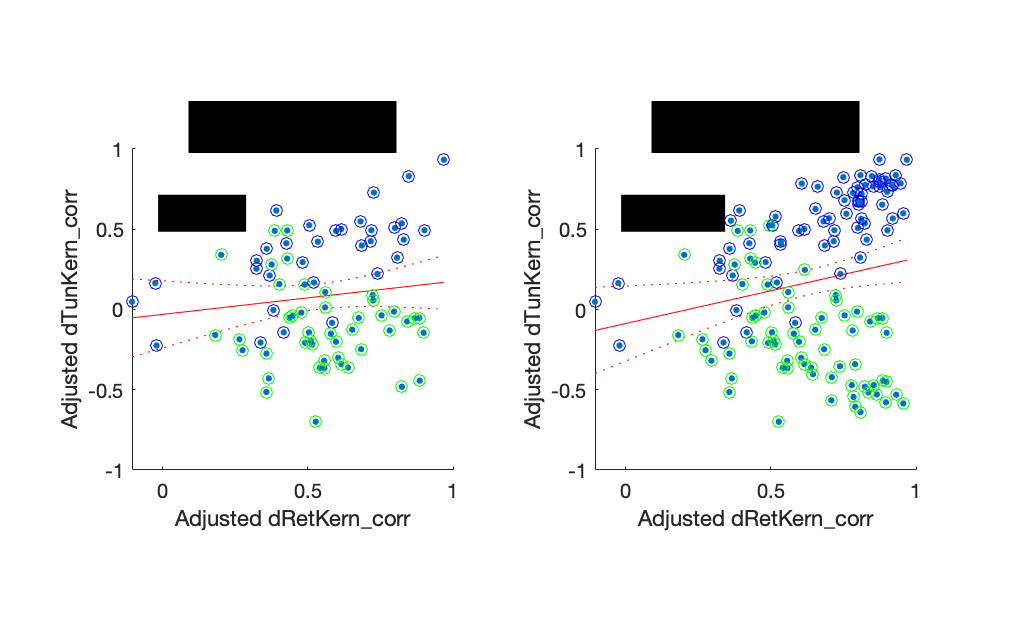
\includegraphics[width=\maxwidth{50.77772202709483em}]{figure_2.png}
\end{center}


\label{H_294C9A6B}
\matlabheading{Discussion}


\begin{matlabcode}
livescript2markdown('lgnTUTORIAL.mlx')
\end{matlabcode}


\label{T_940C3757}
\vspace{1em}

\end{document}
